Here first the limitations of Scikit-learn predefined ML models - Logistic Regression(LR) and Multi-Layer-Perceptron(MLP), are described. The Logistic Regression Model seems to work almost perfectly with all 3 classes when the bad region size is $5\times5$ (as in \autoref{Occupancymaps5x5}) with either the same or randomized location. When the bad region size is 1x1 like in \autoref{Ocuppancymaps1x1} the LR Model performs poorly with an accuracy of approximately 20\%.
 The MLP does not seem to work in any of the used cases that are studied as it always performs poorly with an accuracy of $\approx 40\%$.

\begin{figure}[h]
\centering
\begin{subfigure}[t]{.316\textwidth}
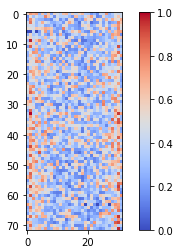
\includegraphics[width=\textwidth]{Good_image_1x1.png}
\caption{}
\end{subfigure}
\begin{subfigure}[t]{.305\textwidth}
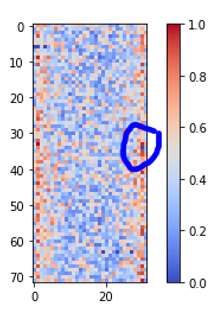
\includegraphics[width=\textwidth]{Dead_image_1x1.png}
\caption{}
\end{subfigure}
\begin{subfigure}[t]{.3\textwidth}
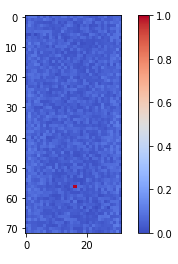
\includegraphics[width=\textwidth]{Hot_image_1x1.png}
\caption{}
\end{subfigure}
\vspace{5mm}
\caption{Occupancy Maps with 1x1 bad regions. A) Good image B) Dead image C) Hot image\label{Ocuppancymaps1x1}}
\end{figure}

Also, the use of Scikit-learn’s library is limited in comparison with the Keras module since one cannot customize the structure of the ML model with detail. Moreover, Keras is an ML library designed for developing deep neural networks. Hence it was decided to use Keras primarily for the creation of the model.
 With the Keras library, numerous models were designed with both, SL method and SSL learning method. Using SL method, we are interested in detecting anomalies and classifying what type of anomaly is seen. With SSL method, we are interested in looking at the error of the reconstruction of an image to give an idea that the image given can be considered good or that it might have some unseen anomalies

\section{SL Models for known anomalies in the HCAL data for DQM}
We considered three SL Models for classification of known anomalies in the HCAL data for DQM. 
These models are based on Convolutional Neural Networks and differ in the number of layers utilized, their ordering and number of units in each layer. The Models and the corresponding results are described below.


\subsection{Two Convolutional Layers for binary classification}
Several variations of the two Convolutional Layers Model were tested and optimized on the DQM data. This led to an optimal value of 8 units/neurons in the Convolutional layers. 
The detail of selecting the number of units per layer is of great importance to find a balance between efficiency and complexity of a model. More complex models (more layers and connections) are “heavy” to train in terms of computational cost, provide better results and are prone to “overfitting” to the training data.
 Simpler models (fewer layers and connections) are quicker to train, efficient and computationally economic. However, simpler models are more likely to “underfit” to the data. The \autoref{fig:2convlayermodel} below shows a code snippet with this model.
\autoref{fig:2convlayermodelfixedresults} below shows the learning curve for this model trained with Good and Hot images for fixed $5\times 5$ location and the corresponding Confusion Matrix.

\autoref{fig:2convlayermodelrandomresults} shows the learning curve for this model trained with Good and Hot images for fixed 5x5 location and the corresponding Confusion Matrix.

\begin{figure}
\begin{center}
    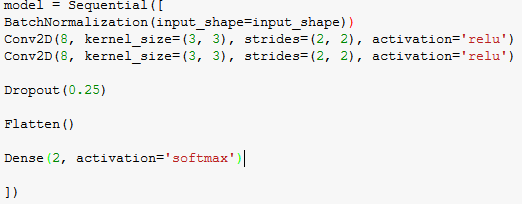
\includegraphics[width=.9\textwidth]{2_conv_layers_model.png}
\end{center}
\caption{Two Convolutional Layers Model\label{fig:2convlayermodel}}
\end{figure}


\begin{figure}
\centering
	\begin{subfigure}{.45\textwidth}
 	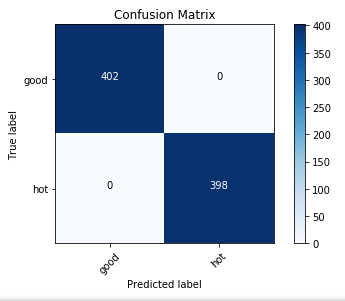
\includegraphics[width=\textwidth]{CM_2x2_with_5x5_good_hot_fixed.png}
	\end{subfigure}
	\begin{subfigure}{.45\textwidth}
	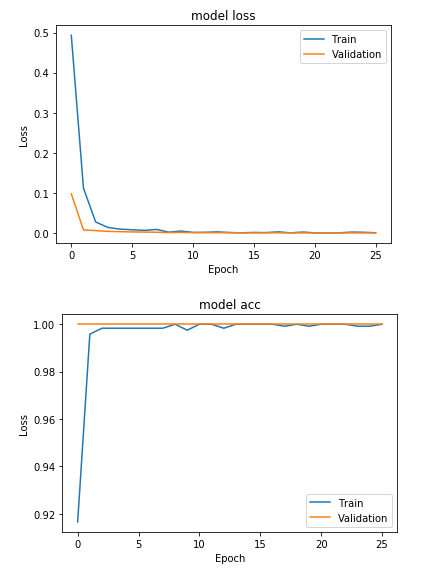
\includegraphics[width=\textwidth]{Learning_curve_5x5_good_hot_fixed.png}
	\end{subfigure}
	\caption{Confusion Matrix results and Learning curve
	 for $5\times 5$ damaged area with on the same location for all trials\label{fig:2convlayermodelfixedresults}}
 \end{figure}
 
 \begin{figure}
 	\begin{subfigure}{.45\textwidth}
 		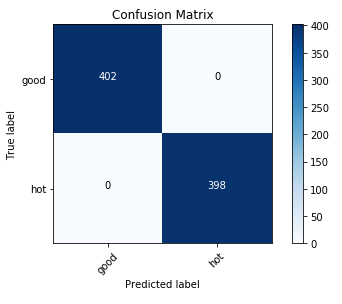
\includegraphics[width=\textwidth]{2x2CMwith_5x5_good_hot_random.png}
 	\end{subfigure}
 	\begin{subfigure}{.45\textwidth}
 	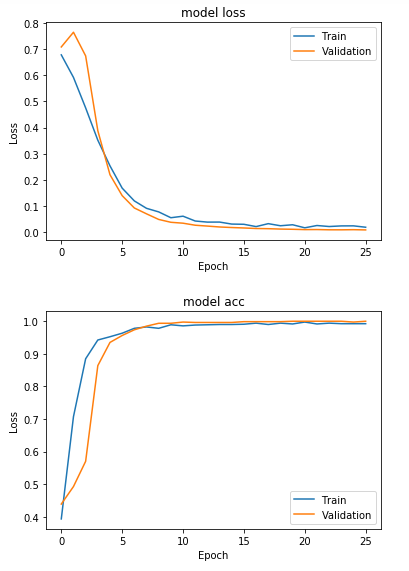
\includegraphics[width=\textwidth]{Learning_curve_5x5_good_hot_random.png}
 	\end{subfigure}
 \caption{Confusion Matrix results and Learning curve
	 for $5\times5$ damaged area with on the random location for all trials\label{fig:2convlayermodelrandomresults}}
 \end{figure}
 

\begin{figure}
	\begin{subfigure}{.495\textwidth}
 		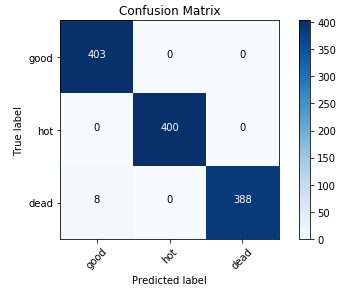
\includegraphics[width=\textwidth]{3x3CMwith_5x5_good_hot_dead_random.png}
 	\end{subfigure}
 	\begin{subfigure}{.45\textwidth}
 	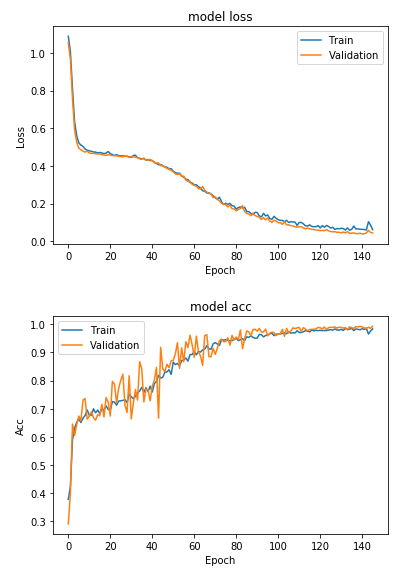
\includegraphics[width=\textwidth]{Learning_curve_5x5_good_hot_dead_random.png}
 	\end{subfigure}
 \caption{Confusion Matrix results and Learning curve
	 for $5\times5$ damaged area with an extra class to identify with random location for all trials\label{fig:2convlayermodelGHDrandomresults}}
 \end{figure}
 
\autoref{fig:2convlayermodelGHDrandomresults} shows the learning curve for this model trained with Good, Hot and Dead images for random 5x5 location and the corresponding Confusion Matrix

Figure 12 below shows the learning curve for this model trained with Good, Hot and Dead images for random 1x1 location and the corresponding Confusion Matrix. The corresponding learning curves and confusion matrix for a fixed location for 3-class (Good, Hot, Dead) configuration give the same behavior as 2-labels (Good, Hot) images



\begingroup
	\large
	\begin{center}
	%\begin{equation}
		$f = \frac{fake}{prompt+fake}$ ,
	\end{center}
	%\end{equation}
\endgroup
\vspace{1em}

\autoref{FakeRatePurityLoose} shows the purity and fakerate for photons that pass the loose ID/selection, have a $p_\text{T} > 200$ GeV and are within the ECAL acceptance range. A sample is obtained in which 77\% of the photons are direct, 12\% are fragmentation and 11\% are fakes. This implies an average purity of $\sim$89\% for this sample, well within the value that is expected. \autoref{FakeRatePurityCR} shows the same ratios for the loose $\gamma$+ jets control region described in \autoref{photonSelection}. Although the amount of statistics has decreased due to the additional cuts, a similar trend can be observed.


\begingroup
	\Large
	\begin{center}
	%\begin{equation}
		$S^{i}_{\gamma} = \frac{\text{Data}^{i} - \text{M}\text{C}^{i}_\text{other}}{\text{M}\text{C}_{\gamma+\text{jets}}^i}$,
	\end{center}
	%\end{equation}
\endgroup

\noindent {where i denotes any given bin in the $N_j$ distribution. The shape correction factors $S^{i}_{\gamma}$ are displayed graphically in \autoref{NjetsCR} (right) for each $N_j$ bin. These factors correct for differences in the jet multiplicity shape, while the overall normalization is estimated from the tight $\mu\mu$ control region. \autoref{NjetsShapeCorr} shows the $N_j$ distribution in the tight $\mu\mu$ control region after the calculated scale factors have been applied. The $S_{\gamma}$ correction will be applied to the Z$\rightarrow\nu\bar{\nu}$ simulation final prediction for each of the analysis search bins. The uncertainty associated with the scale factor is estimated from the event yields in the loose photon control region. This uncertainty will form part of the total systematic uncertainty in the final prediction.}

\begin{figure}[H]
\begin{center}
\begin{minipage}[b]{0.45\textwidth}
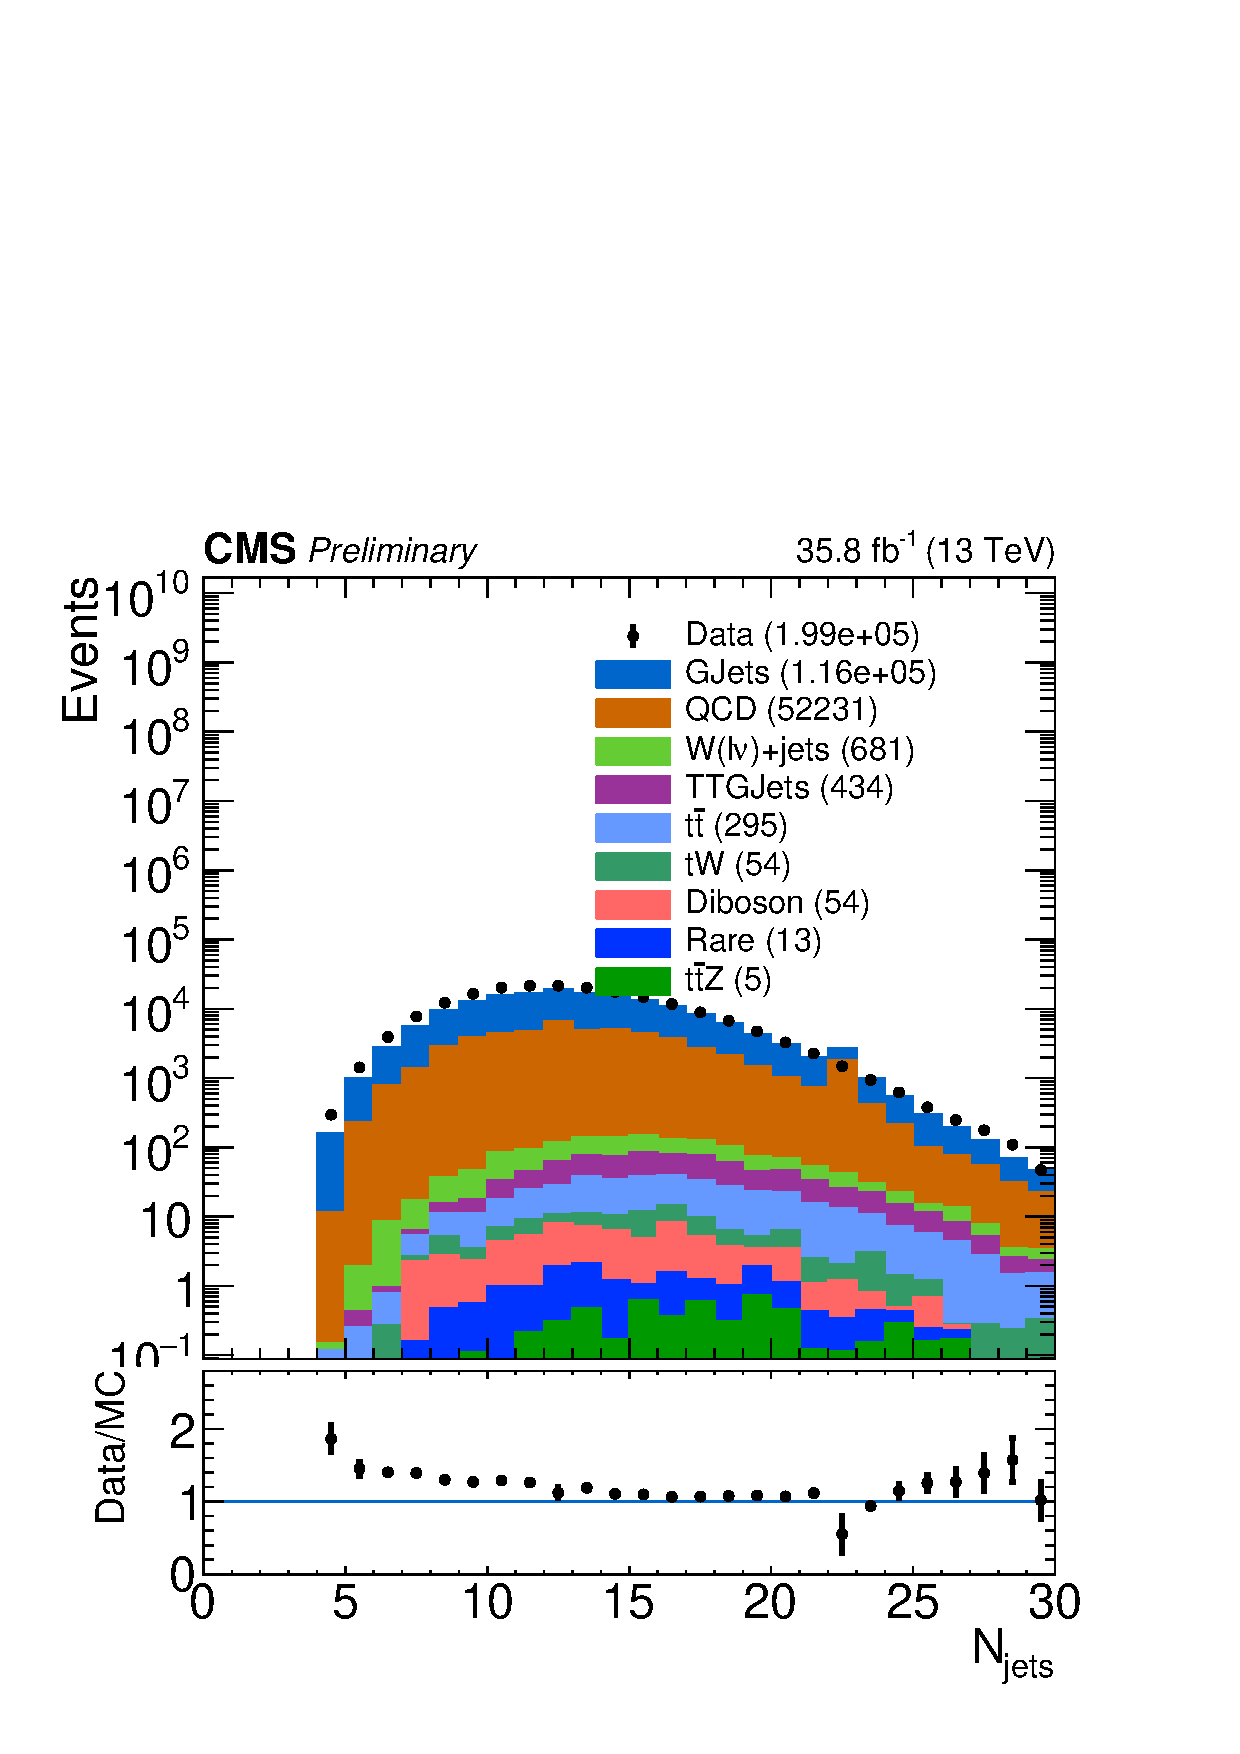
\includegraphics[width=0.94\textwidth]{dataMC_Photon_nj_Log_LooseLepVeto.pdf}
\end{minipage}
\begin{minipage}[b]{0.5\textwidth}
    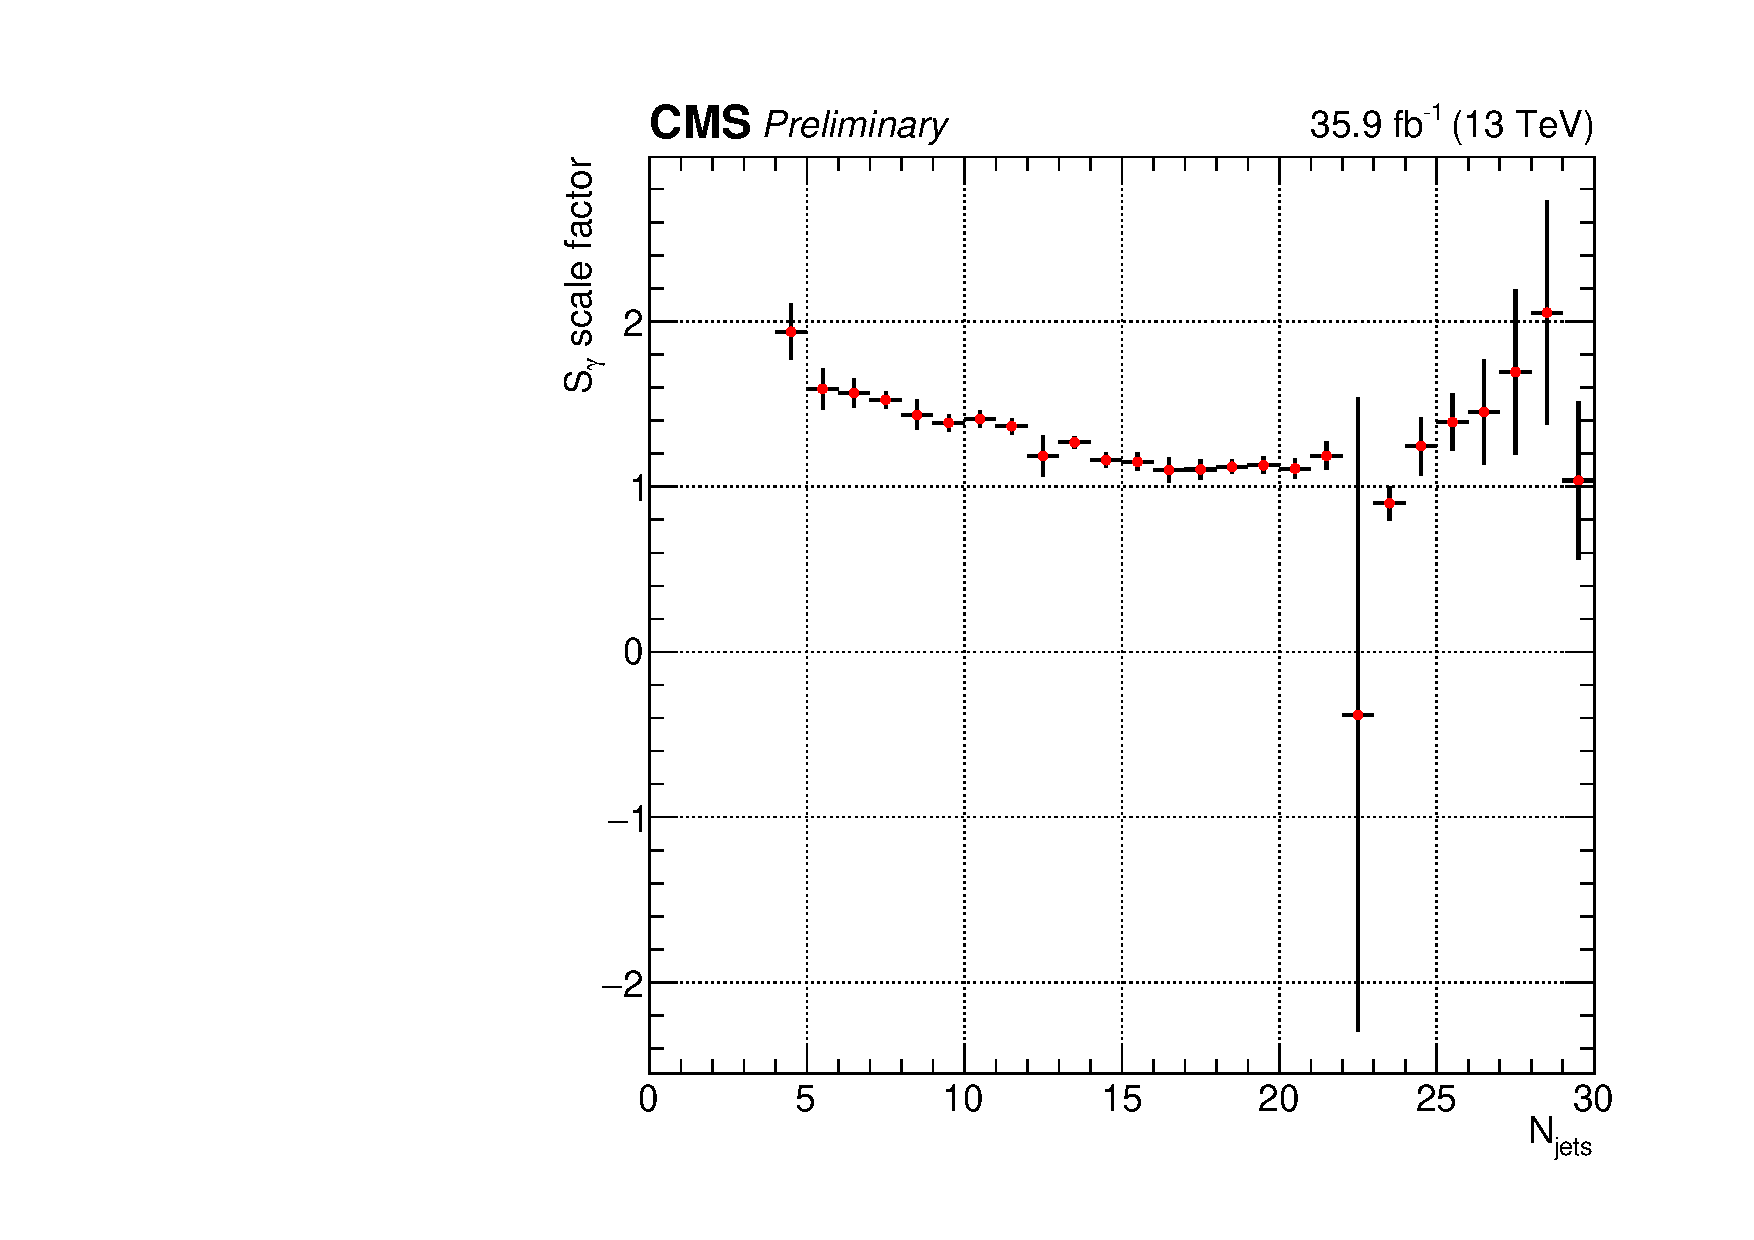
\includegraphics[width=\textwidth]{ShapeCorr_LooseLepVeto.pdf}
\end{minipage}
\end{center}
\vspace{-1em}
\caption{Jet multiplicity and the associated S$_\gamma$ scale factor in the loose photon control region before any corrections are applied.}
\label{NjetsCR}
\end{figure}

%\vspace{1em}

\begin{figure}[H]
\begin{center}
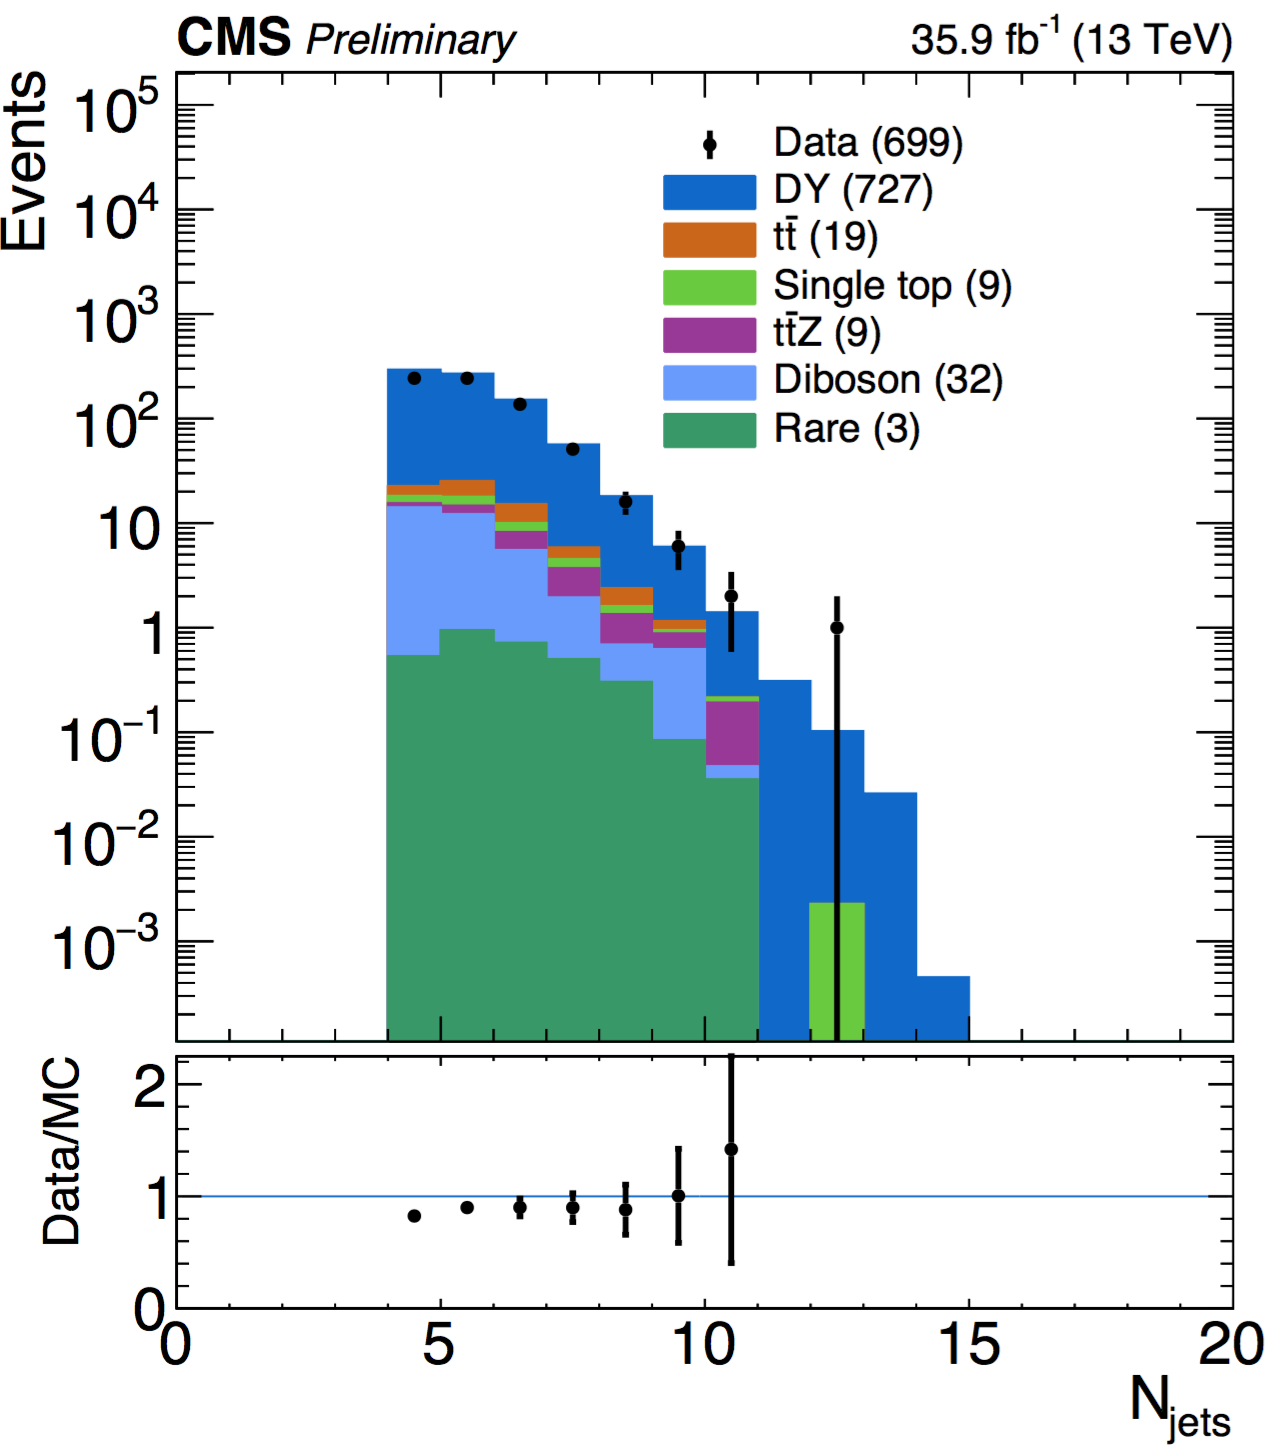
\includegraphics[width=0.4\textwidth]{NjetsShapeCorr.png}
\end{center}
\vspace{-1em}
\caption[$N_{jet}$ distribution in the tight $\mu\mu$ control region after $S_\gamma$ corrections.]{$N_{jet}$ distribution in the tight $\mu\mu$ control region after $S_\gamma$ corrections.}
\label{NjetsShapeCorr}
\end{figure}

The effect of the $S_{\gamma}$($N_j$) scale factor is shown for various distributions. These results show that the overall agreement between data and simulation improves after applying the corresponding shape corrections.

\begin{figure}[H]
\begin{center}
\begin{minipage}[b]{0.45\textwidth}
    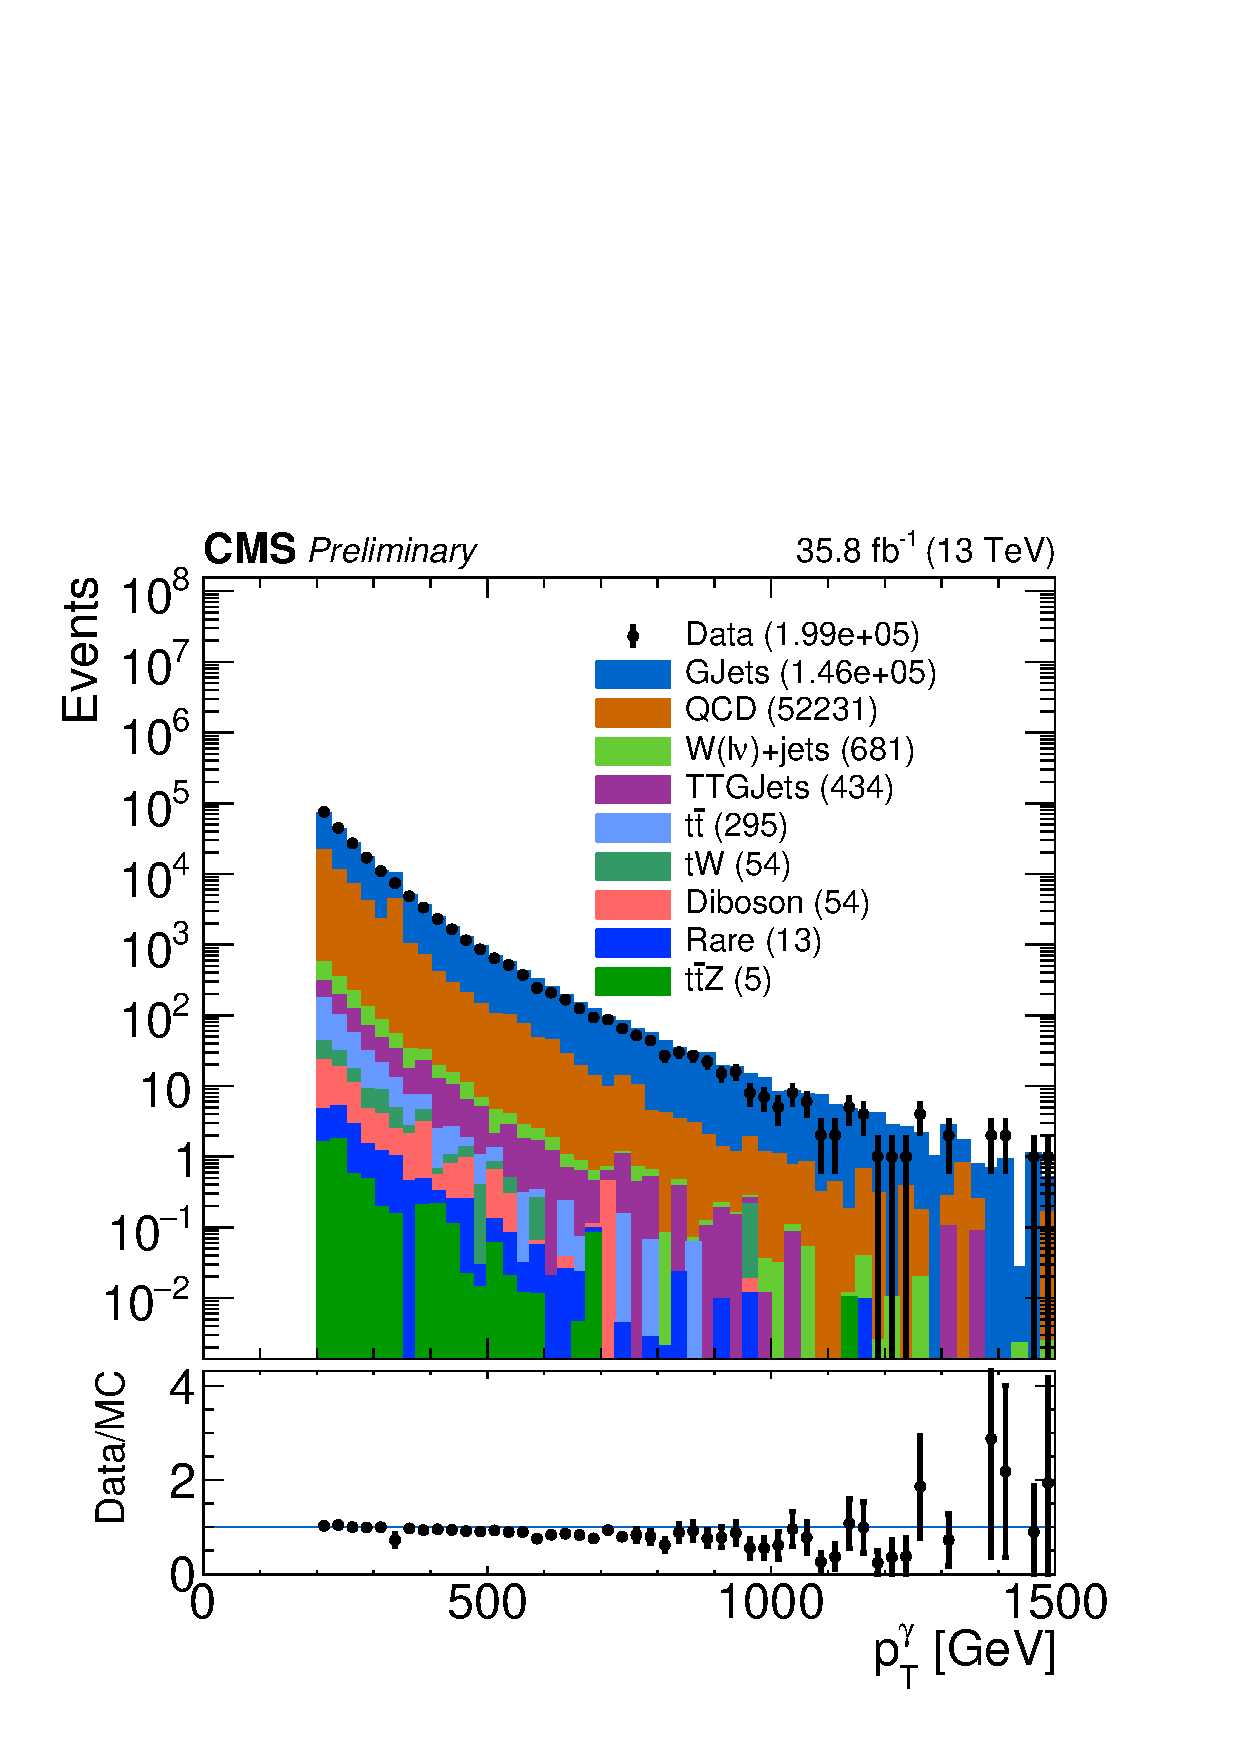
\includegraphics[width=\textwidth]{dataMC_PhotonPt_Wgt_LooseLepVeto.pdf}
\end{minipage}
\begin{minipage}[b]{0.45\textwidth}
    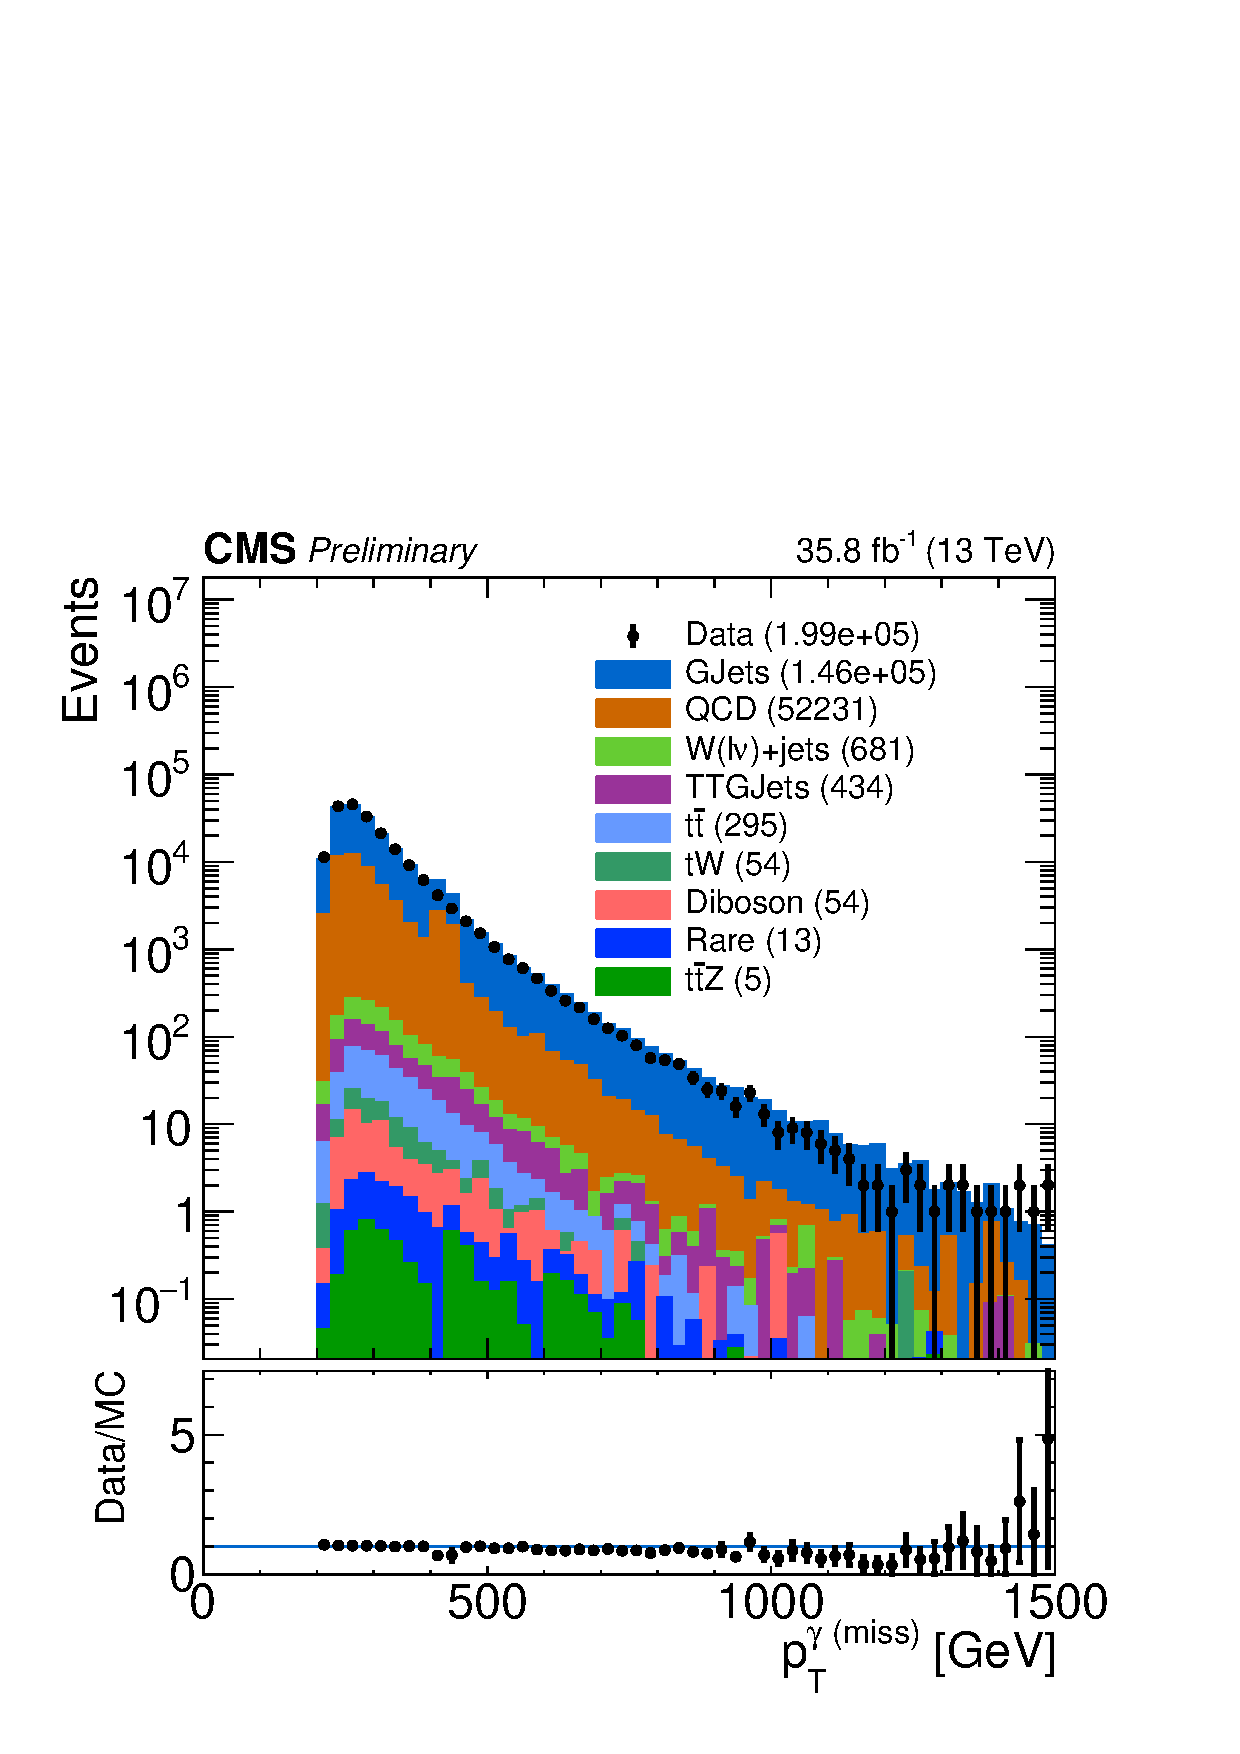
\includegraphics[width=\textwidth]{dataMC_MetGamma_Wgt_LooseLepVeto.pdf}
\end{minipage}
\end{center}
\vspace{-1em}
\caption{$p_\text{T}^\gamma$ (left) and $p_\text{T}^{\gamma (miss)}$ (right) distributions after applying the $S_\gamma$($N_j$) scale factor. Comparing to \autoref{PtMetPt}, an improvement in the agreement between data/MC can be observed.}
\label{PtMetPtCorr}
\end{figure}

\vspace {1em}

\begin{figure}[H]
\begin{center}
\begin{minipage}[b]{0.45\textwidth}
    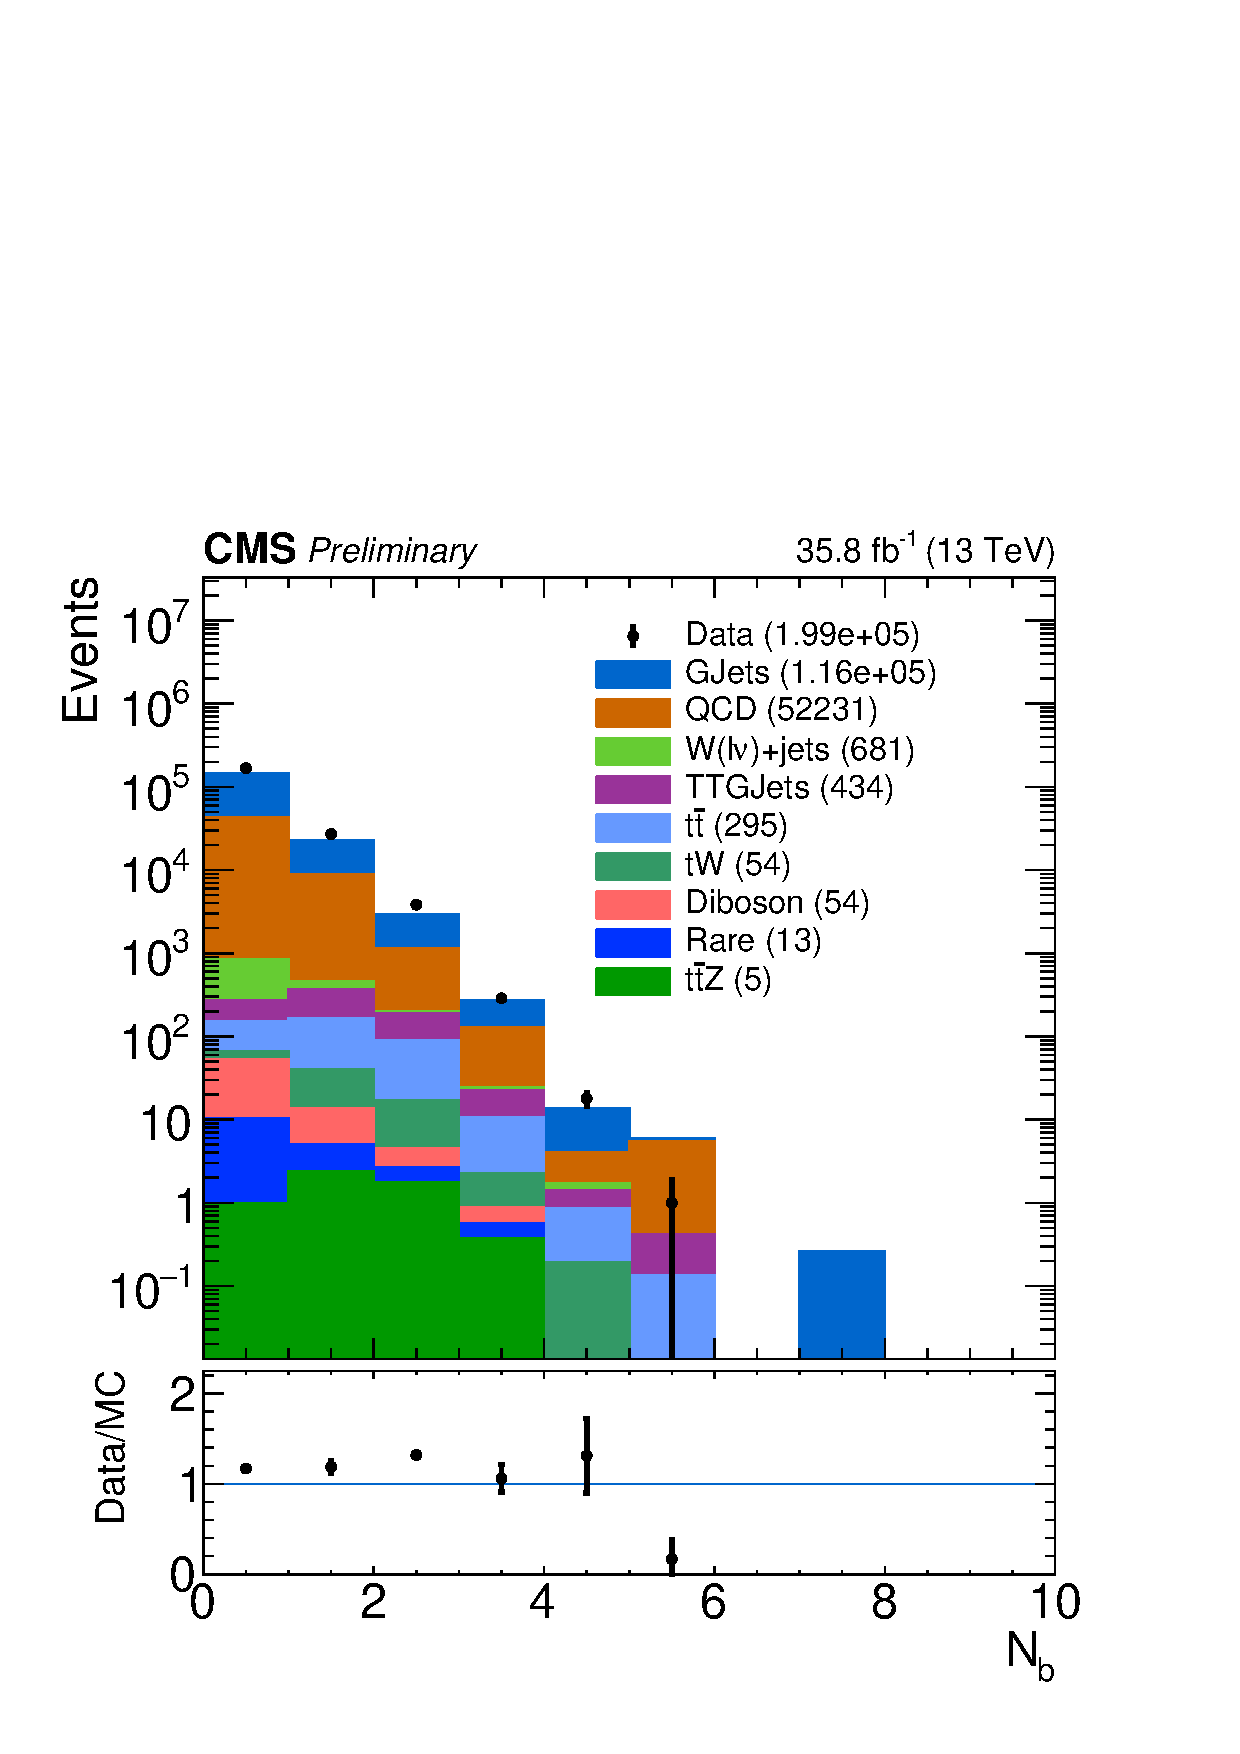
\includegraphics[width=\textwidth]{dataMC_Photon_nb_Log_LooseLepVeto.pdf}
\end{minipage}
\begin{minipage}[b]{0.45\textwidth}
    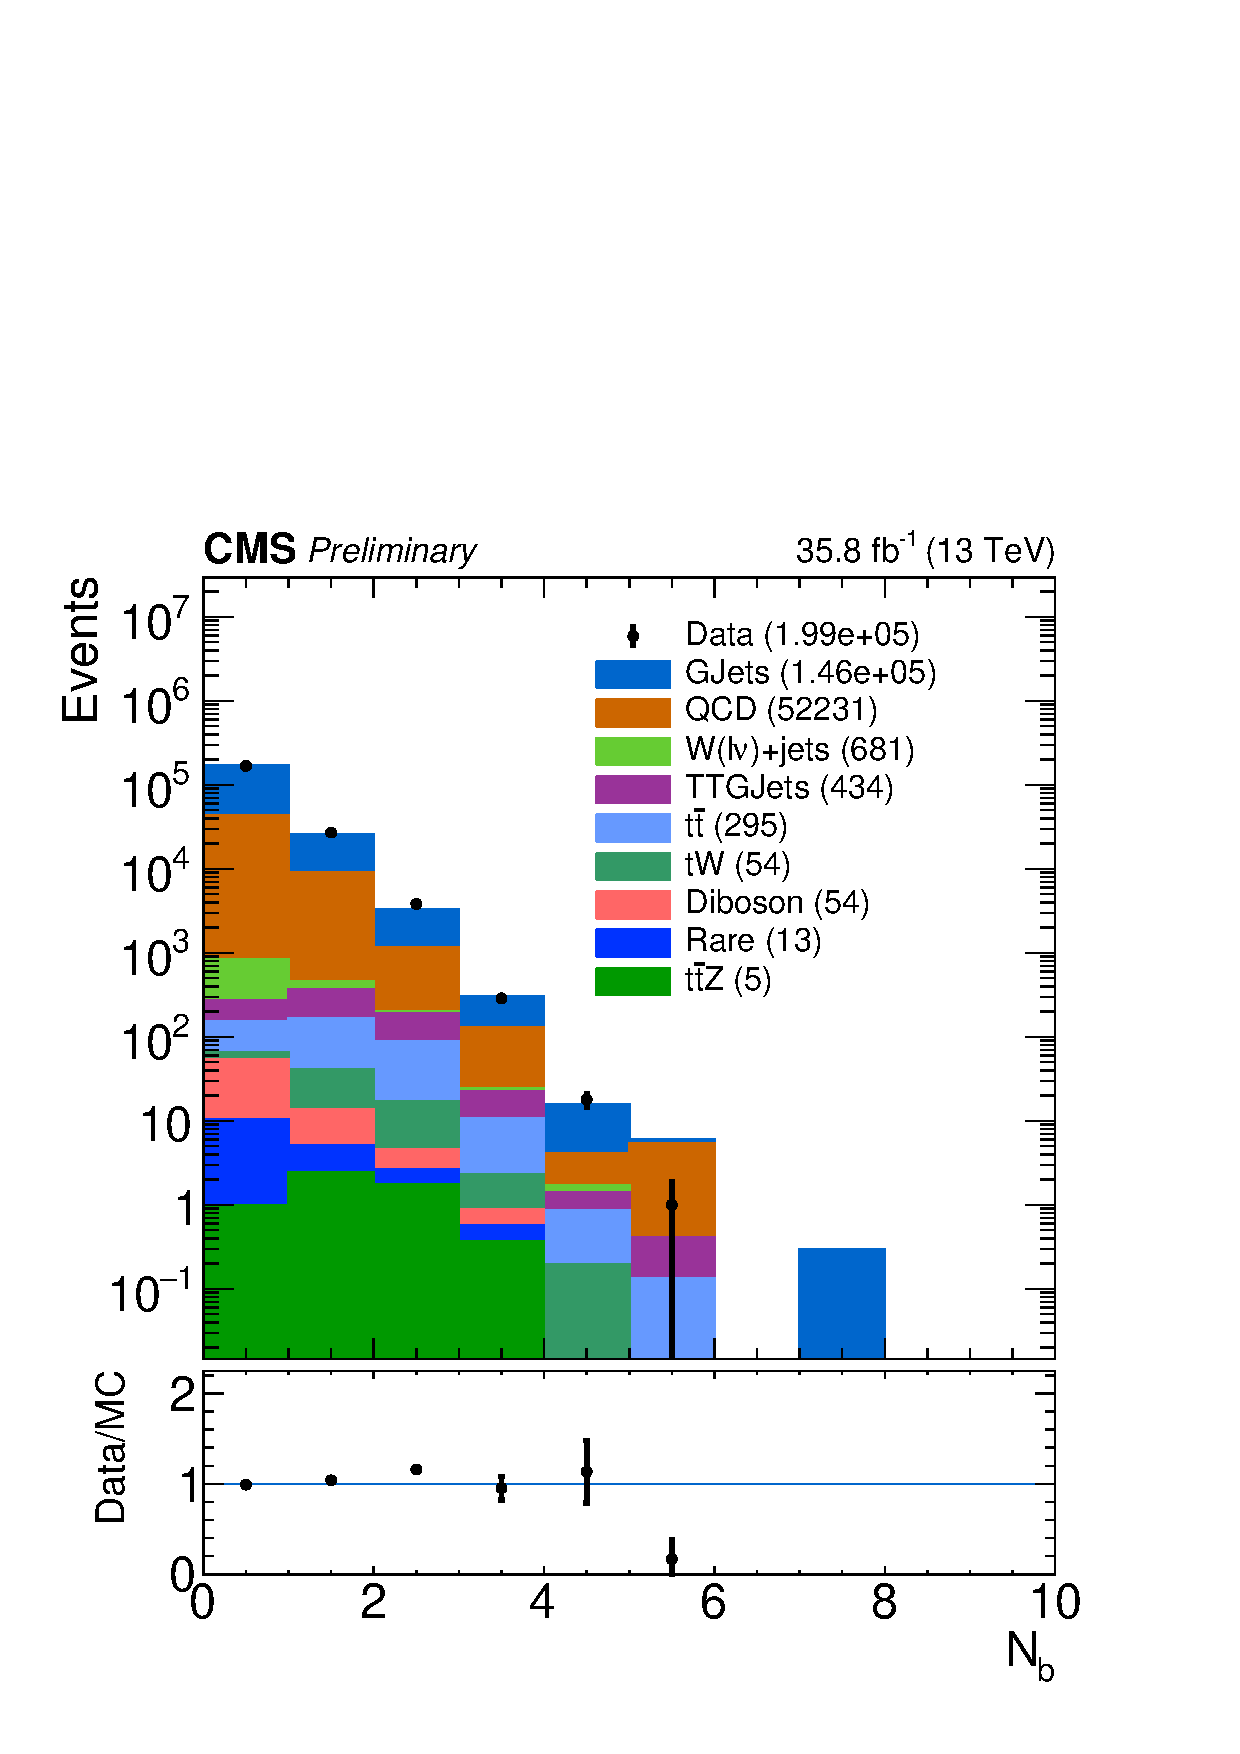
\includegraphics[width=\textwidth]{dataMC_Photon_nb_Log_Wgt_LooseLepVeto.pdf}
\end{minipage}
\end{center}
\vspace{-1em}
\caption{$N_b$ distribution before (left) and after (right) applying the $S_\gamma$($N_j$) scale factor. }
\end{figure}

%\vspace {1em}

\begin{figure}[tb]
\begin{center}
\begin{minipage}[b]{0.45\textwidth}
    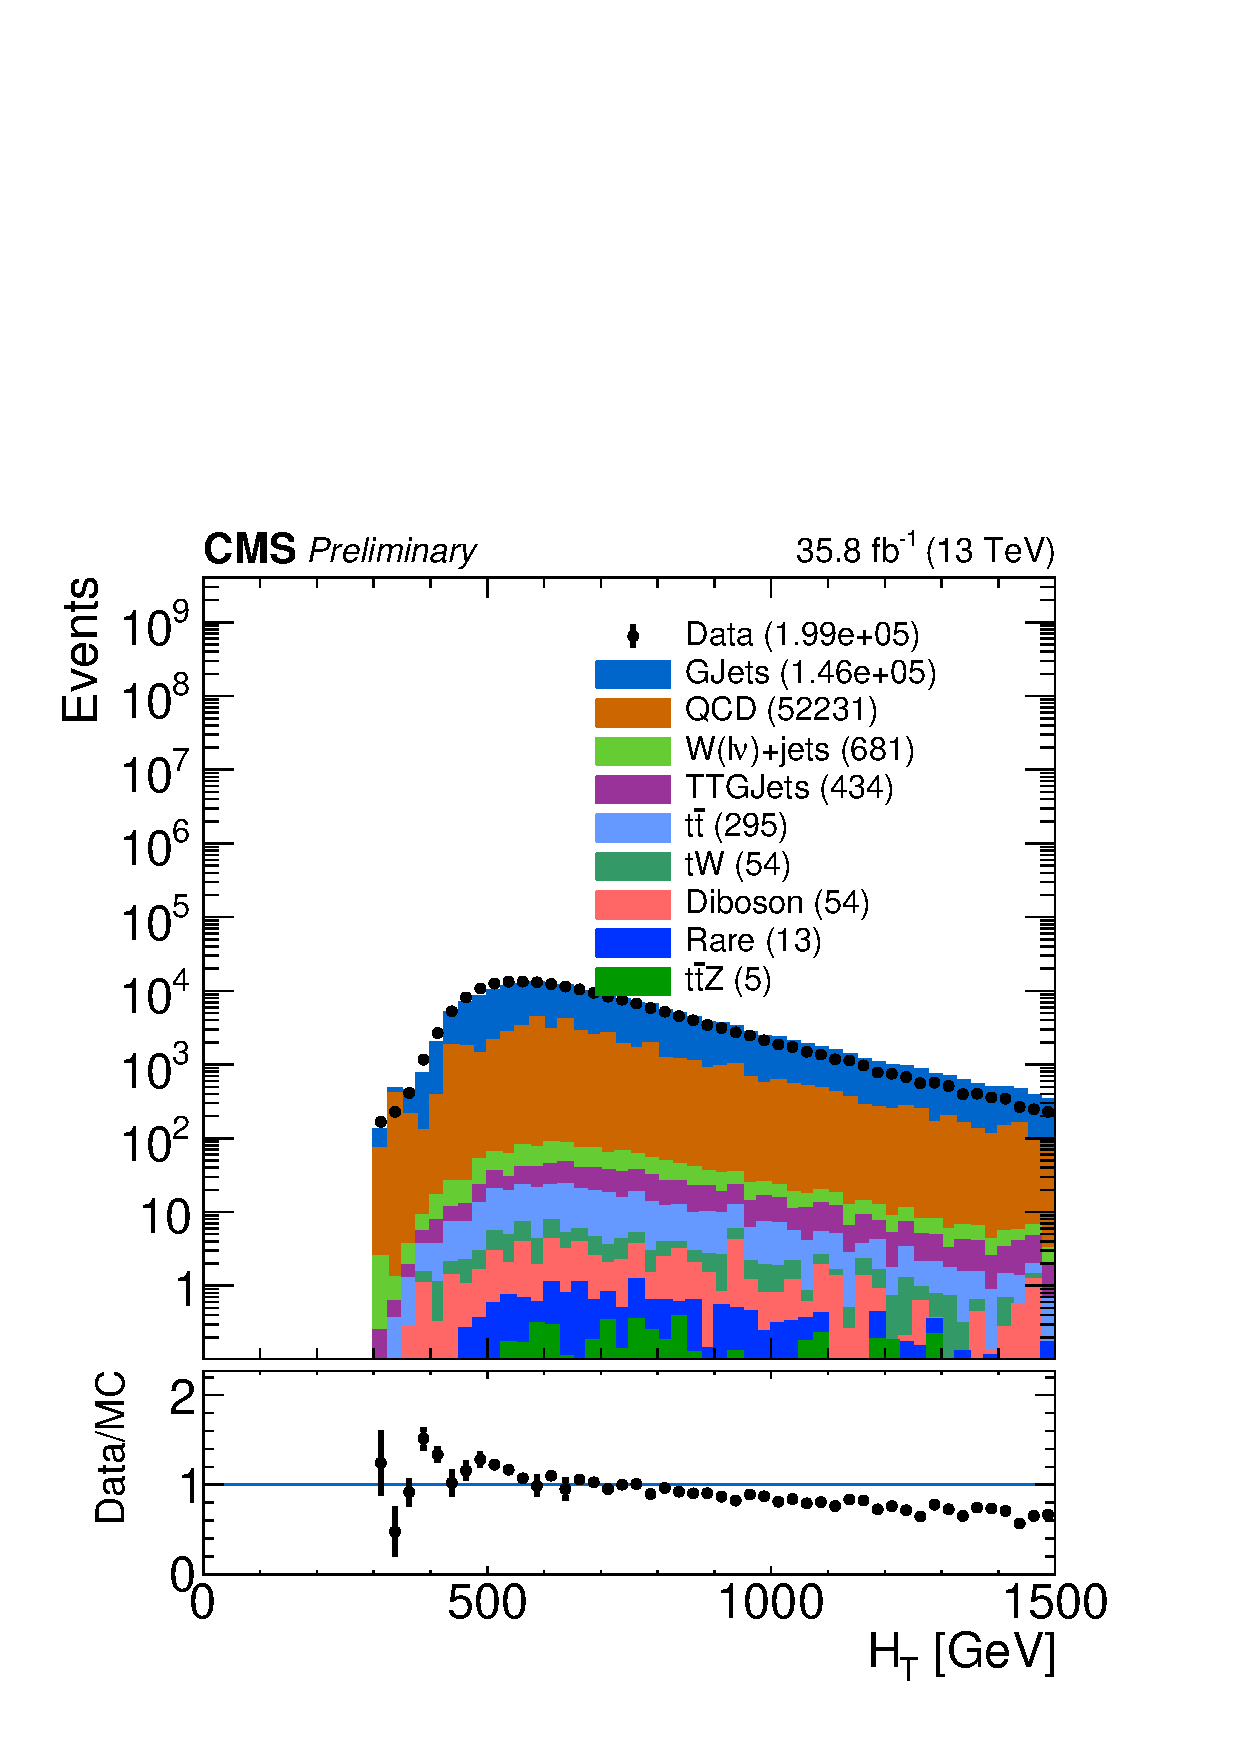
\includegraphics[width=\textwidth]{dataMC_Photon_ht_Wgt_LooseLepVeto.pdf}
\end{minipage}
\begin{minipage}[b]{0.45\textwidth}
    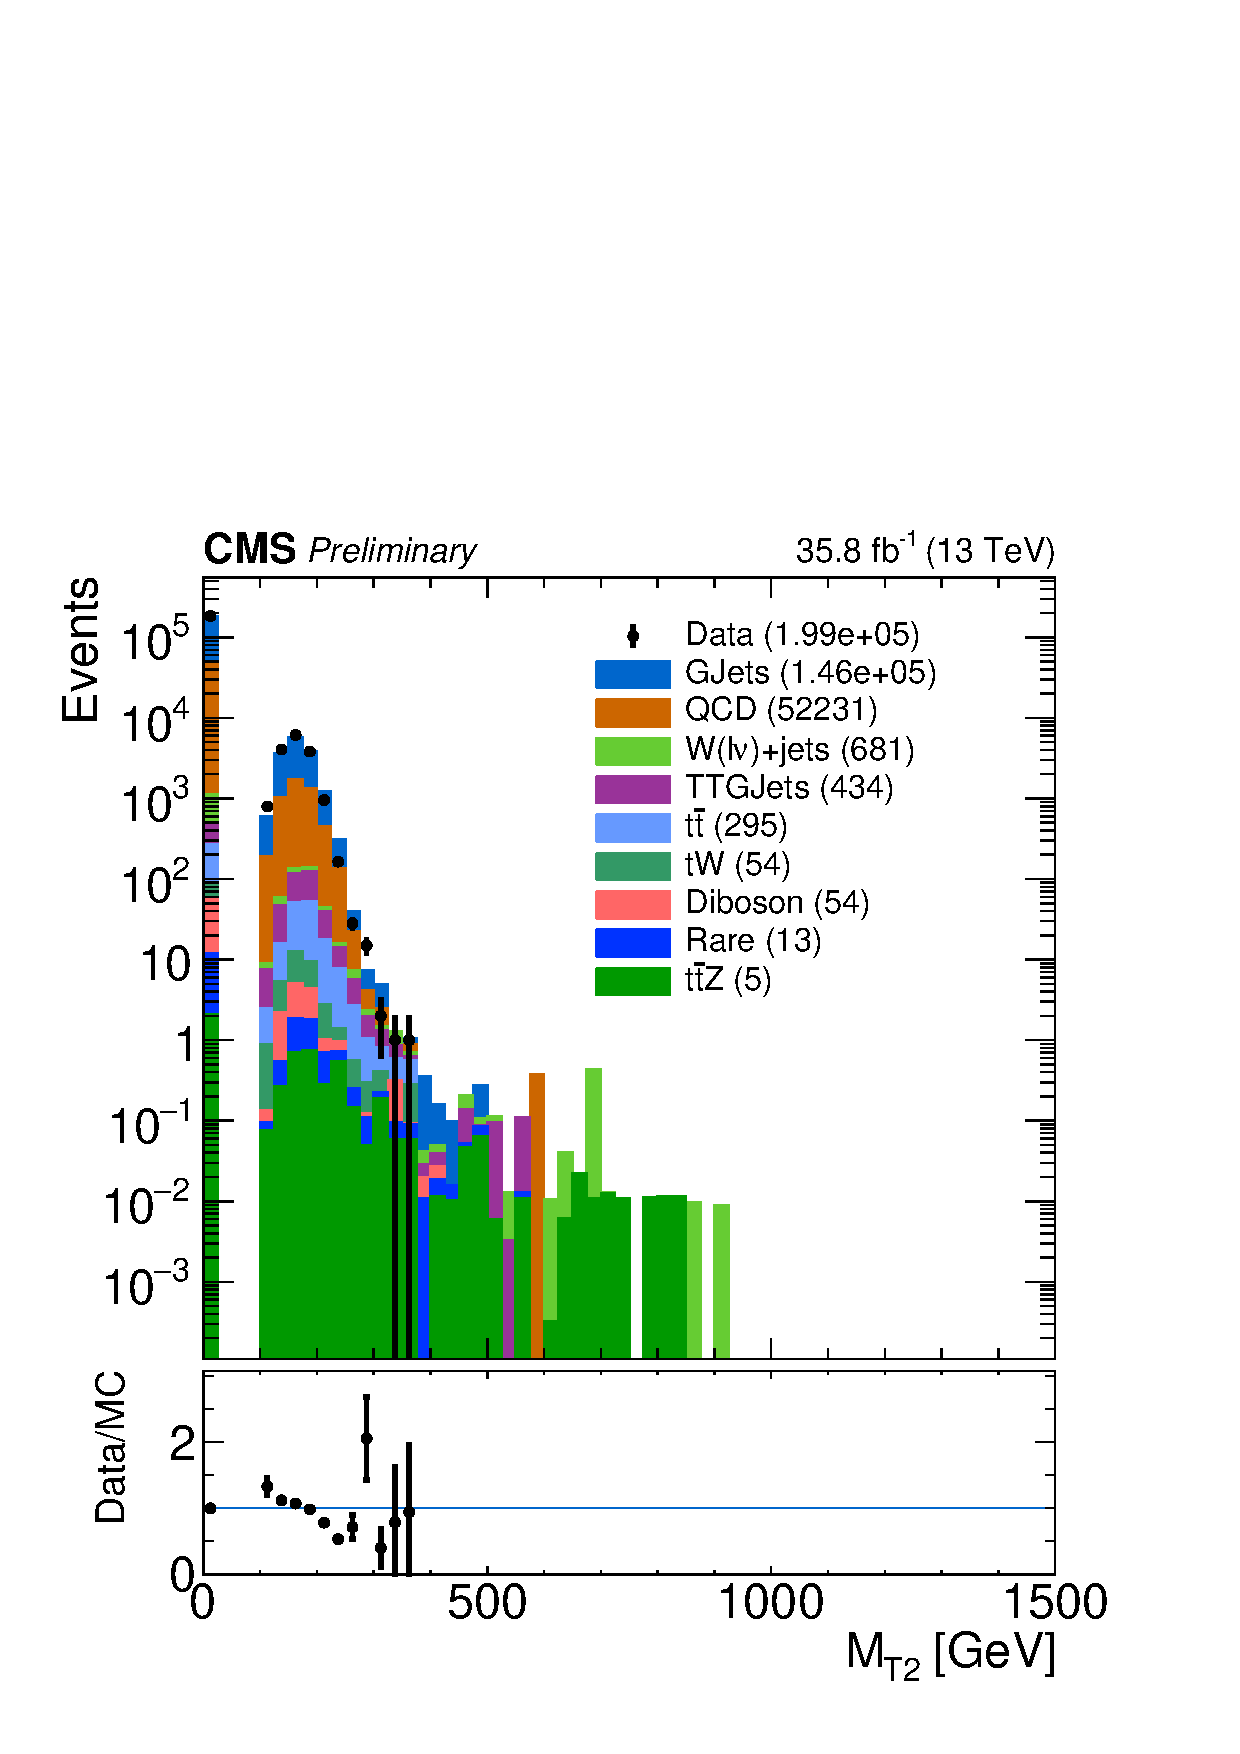
\includegraphics[width=\textwidth]{dataMC_Photon_mt2_Wgt_LooseLepVeto.pdf}
\end{minipage}
\end{center}
\vspace{-1em}
\caption{$H_\text{T}$ and $m_\text{T2}$ distributions applying the $S_\gamma$($N_j$) scale factor. }
\end{figure}

\subsection{Normalization Correction Using the tight Z$\rightarrow\mu^{+}\mu^{-}$ Control Sample}\label{tightmumu}

In order to constrain the normalization of the Z$\rightarrow\nu\bar{\nu}$ simulation sample, a normalization correction factor $R_{norm}$ is calculated from the tight $\mu\mu$ control region defined in \autoref{tightmumu}. Two categories are considered: the zero b-tagged jet category ($N_b = 0$), and the $\geq 1$ b-tagged jet category ($N_b \geq 1$). Both of these categories are statistically consistent with each other but the inclusive region ($N_b \geq 0$) has a lower overall uncertainty. The method used to calculate the normalization scale factor requires that the $N_j$-dependent shape correction factors already be applied. Then, the $R_{norm}$ factor can be extracted from the ratio of the total event yield in data to that in the simulation. This factor is found to be:

\begingroup
	\begin{center}
		$R_{norm} = 1.070 \pm 0.085$,
	\end{center}
\endgroup

\noindent where the uncertainty includes only the associated statistical uncertainties on data and simulation. This uncertainty is found to be propagated to the final background prediction, see \autoref{systematics}.\\

\begin{figure}[H]
\begin{center}
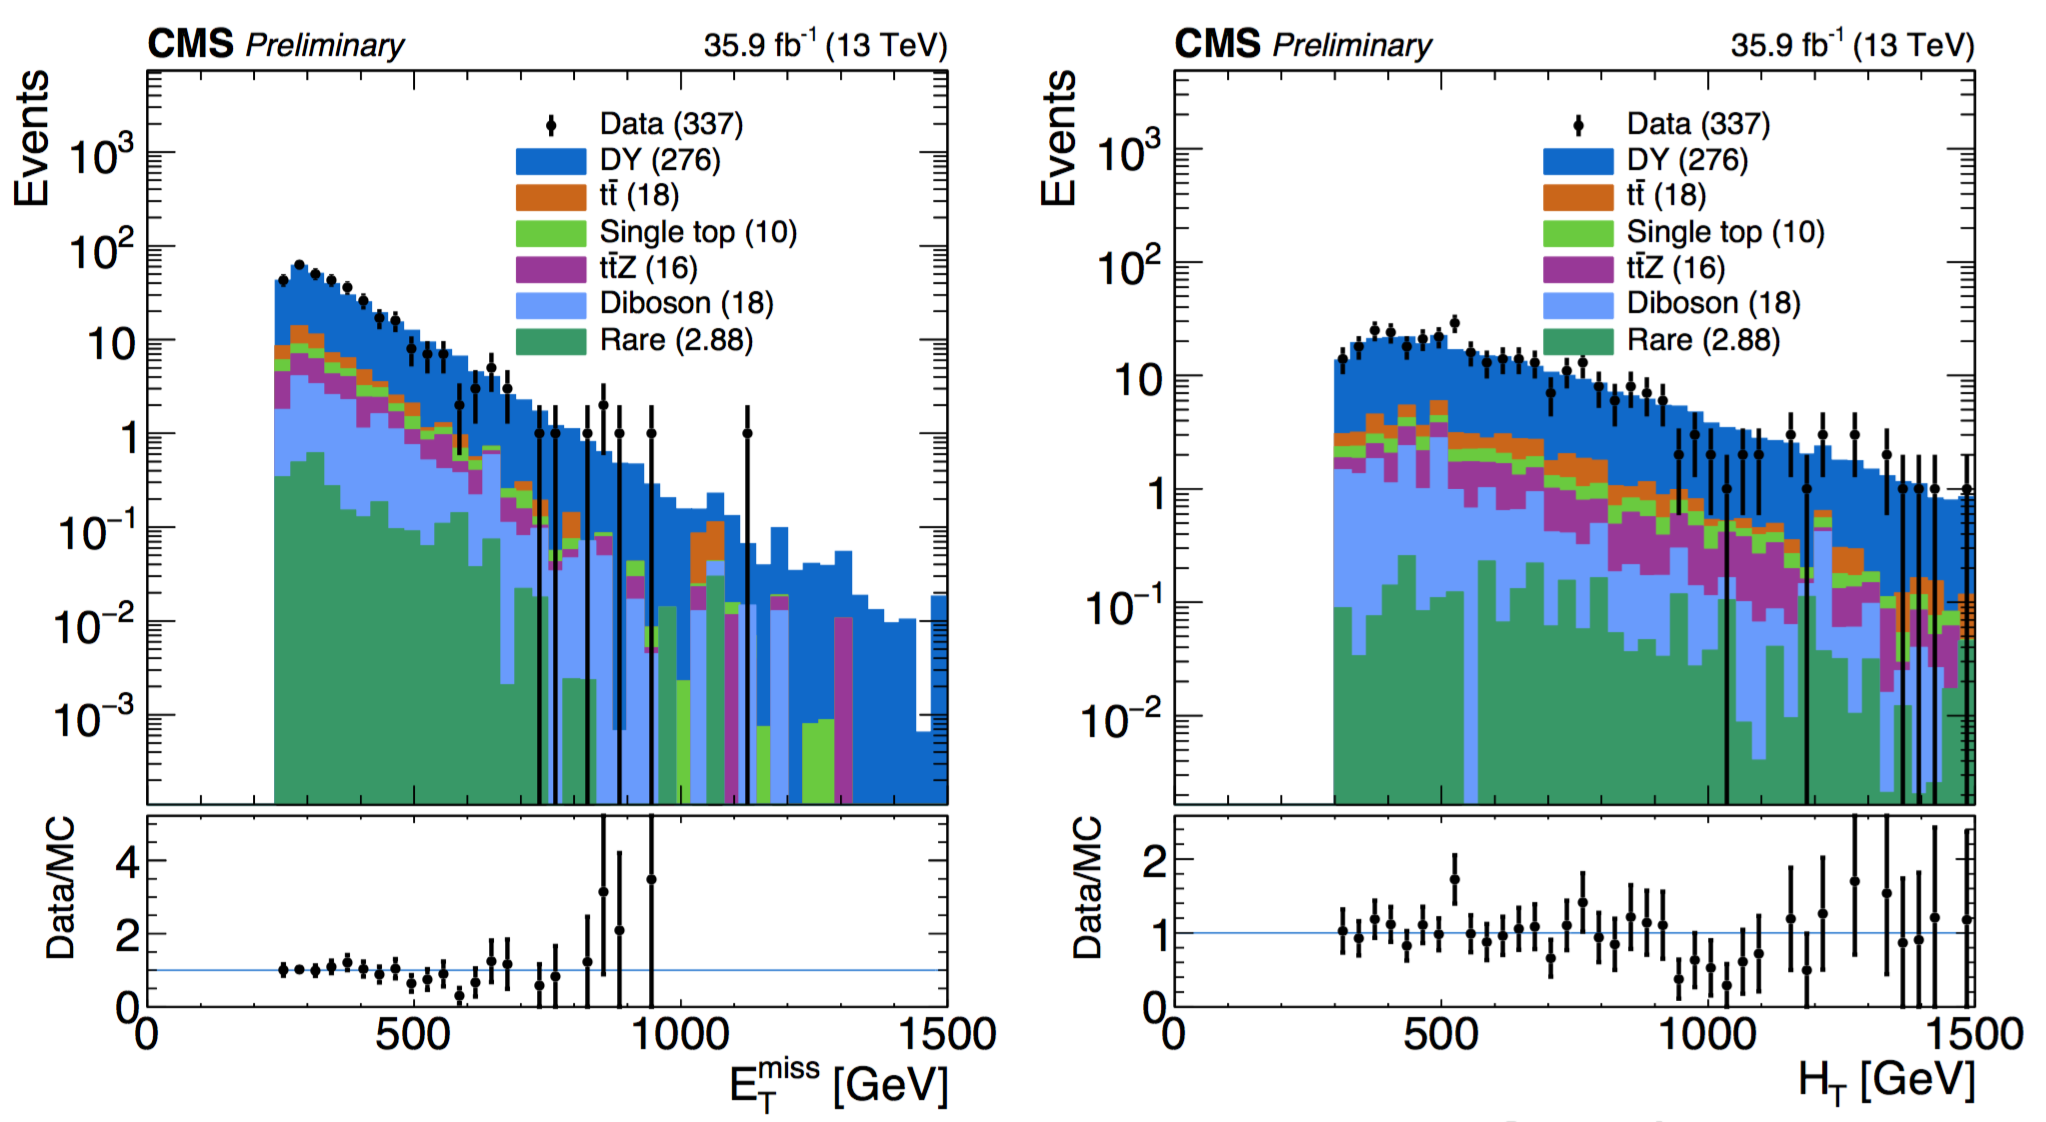
\includegraphics[width=\textwidth]{Rnorm1}
\end{center}
\vspace{-1em}
\caption{Shown are data/MC comparisons for the $p_\text{T}^{miss}$ (left) and $H_\text{T}$ (right) distributions after applying both the $N_j$-dependent shape corrections ($S_\gamma$) and the global normalization scale factor ($R_{norm}$).}
\label{Rnorm1}
\end{figure}

\vspace{1em}

Data/MC comparisons are shown in \autoref{Rnorm1} and \autoref{Rnorm2} after applying $R_{norm}$ for several distributions in the study. With this final global scale factor all the required ingredients for the central value of the Z$\rightarrow\nu\bar{\nu}$ background prediction are obtained. 

\begin{figure}[H]
\begin{center}
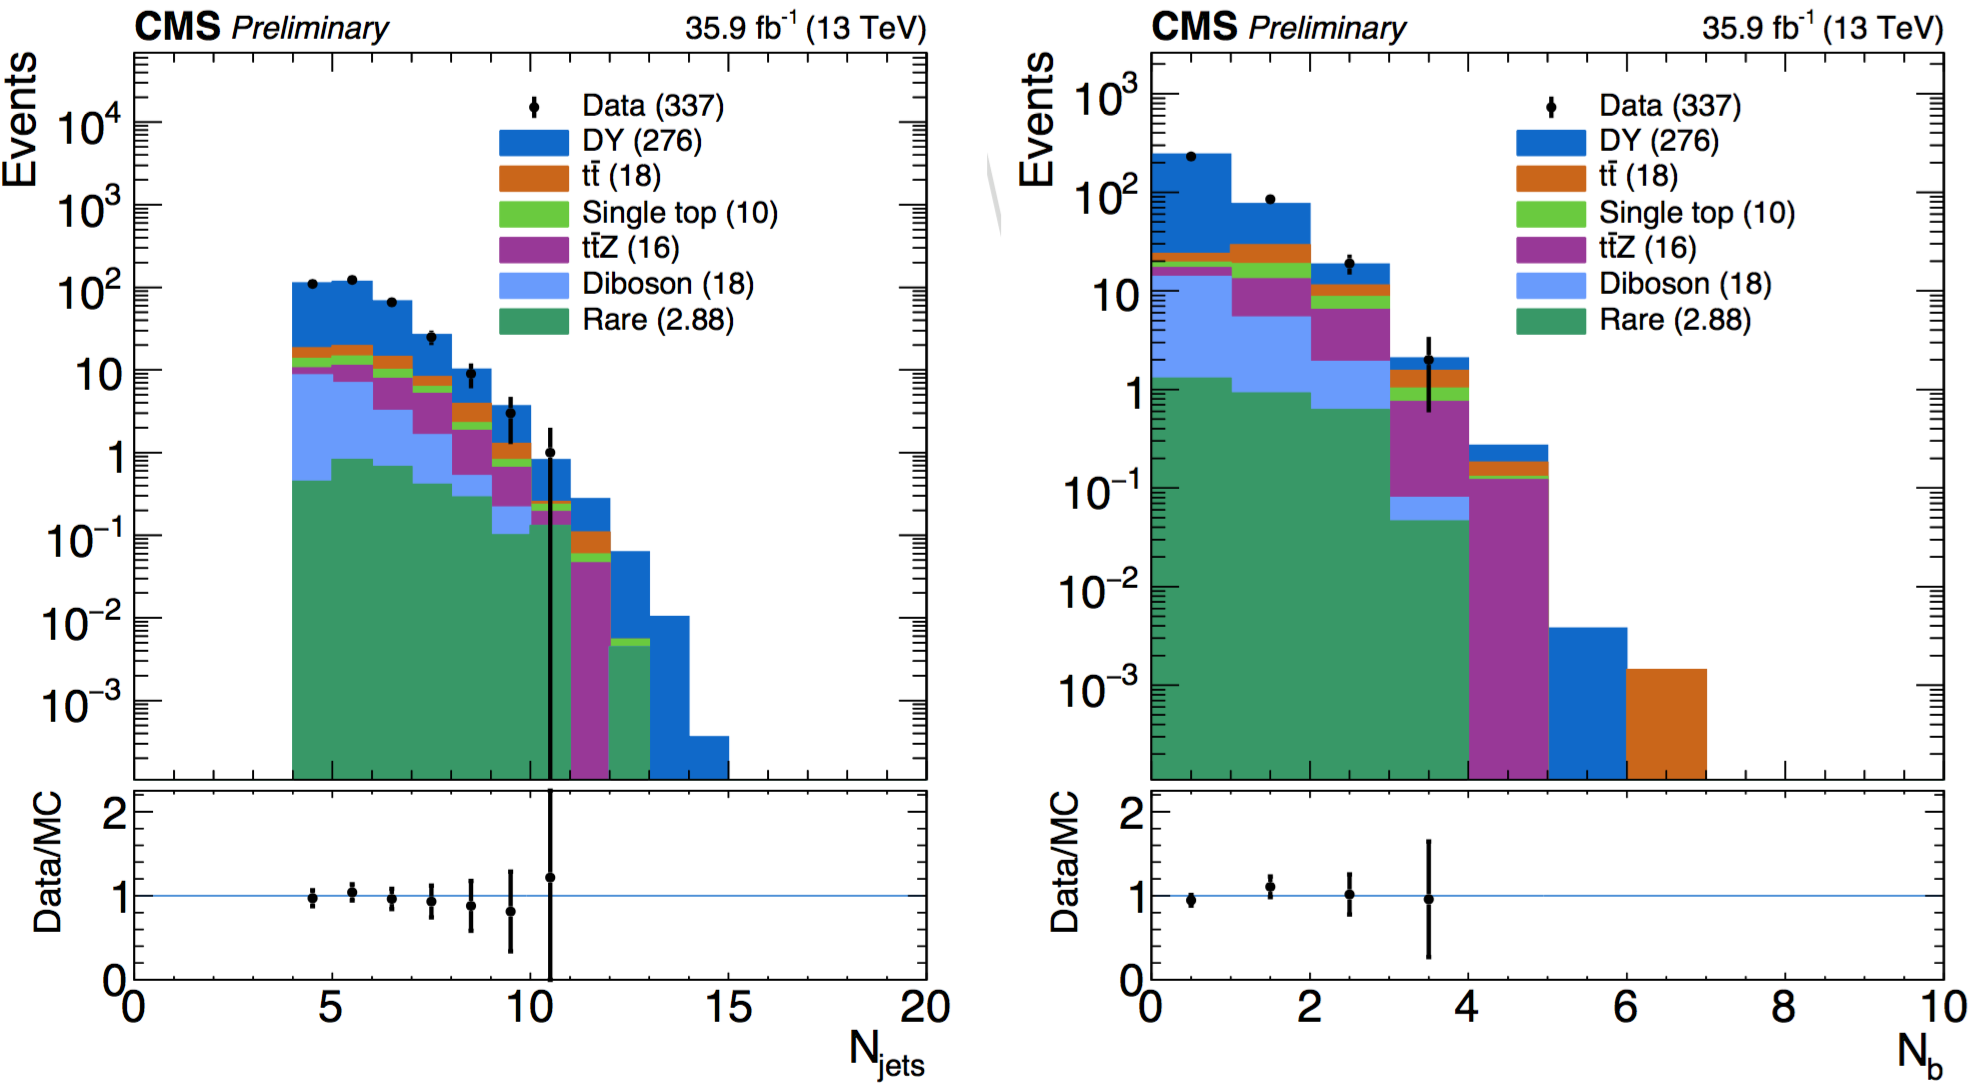
\includegraphics[width=\textwidth]{Rnorm2}
\end{center}
\vspace{-1em}
\caption{Shown are data/MC comparisons for the $N_j$ (left) and $N_b$ (right) distributions after applying both the $N_j$-dependent shape corrections ($S_\gamma$) and the global normalization scale factor ($R_{norm}$).}
\label{Rnorm2}
\end{figure}

\section{Results}

In this section the results for the final estimation of the of the Z$\rightarrow\nu\bar{\nu}$ are presented. The current study includes preliminary results using only data obtained at the CMS detector during 2016. The results for this study are intended to confirm the assumption that the additional $\gamma+$jets control region introduced in this analysis reduce the overall uncertainties obtained in the 2016 analyses (described in \autoref{AnalysisChap}). Furthermore, this study is intended as a benchmark for future analyses of the SUSY stop group based in Fermilab and will be the method used for the 2017 CMS data.

\subsection{Systematics}\label{systematics}

Two categories of uncertainties for the Z$\rightarrow\nu\bar{\nu}$ prediction are considered: uncertainties that are associated to the use of MC simulation and the uncertainties specifically associated to the background prediction method. Several sources are acknowledged in the first category mentioned such as PDF and renormalization/factorization scale choices, jet and $p_\text{T}^{miss}$ energy scale uncertainties b-tag scale factor uncertainties, and trigger efficiency uncertainties. Given that the simulation sample is normalized to data in the tight control region, uncertainties associated with the luminosity and cross-section are excluded. In addition, the overall Z$\rightarrow\nu\bar{\nu}$ statistical uncertainty from MC simulation is also taken into account.\\

\begin{figure}[H]
\begin{center}
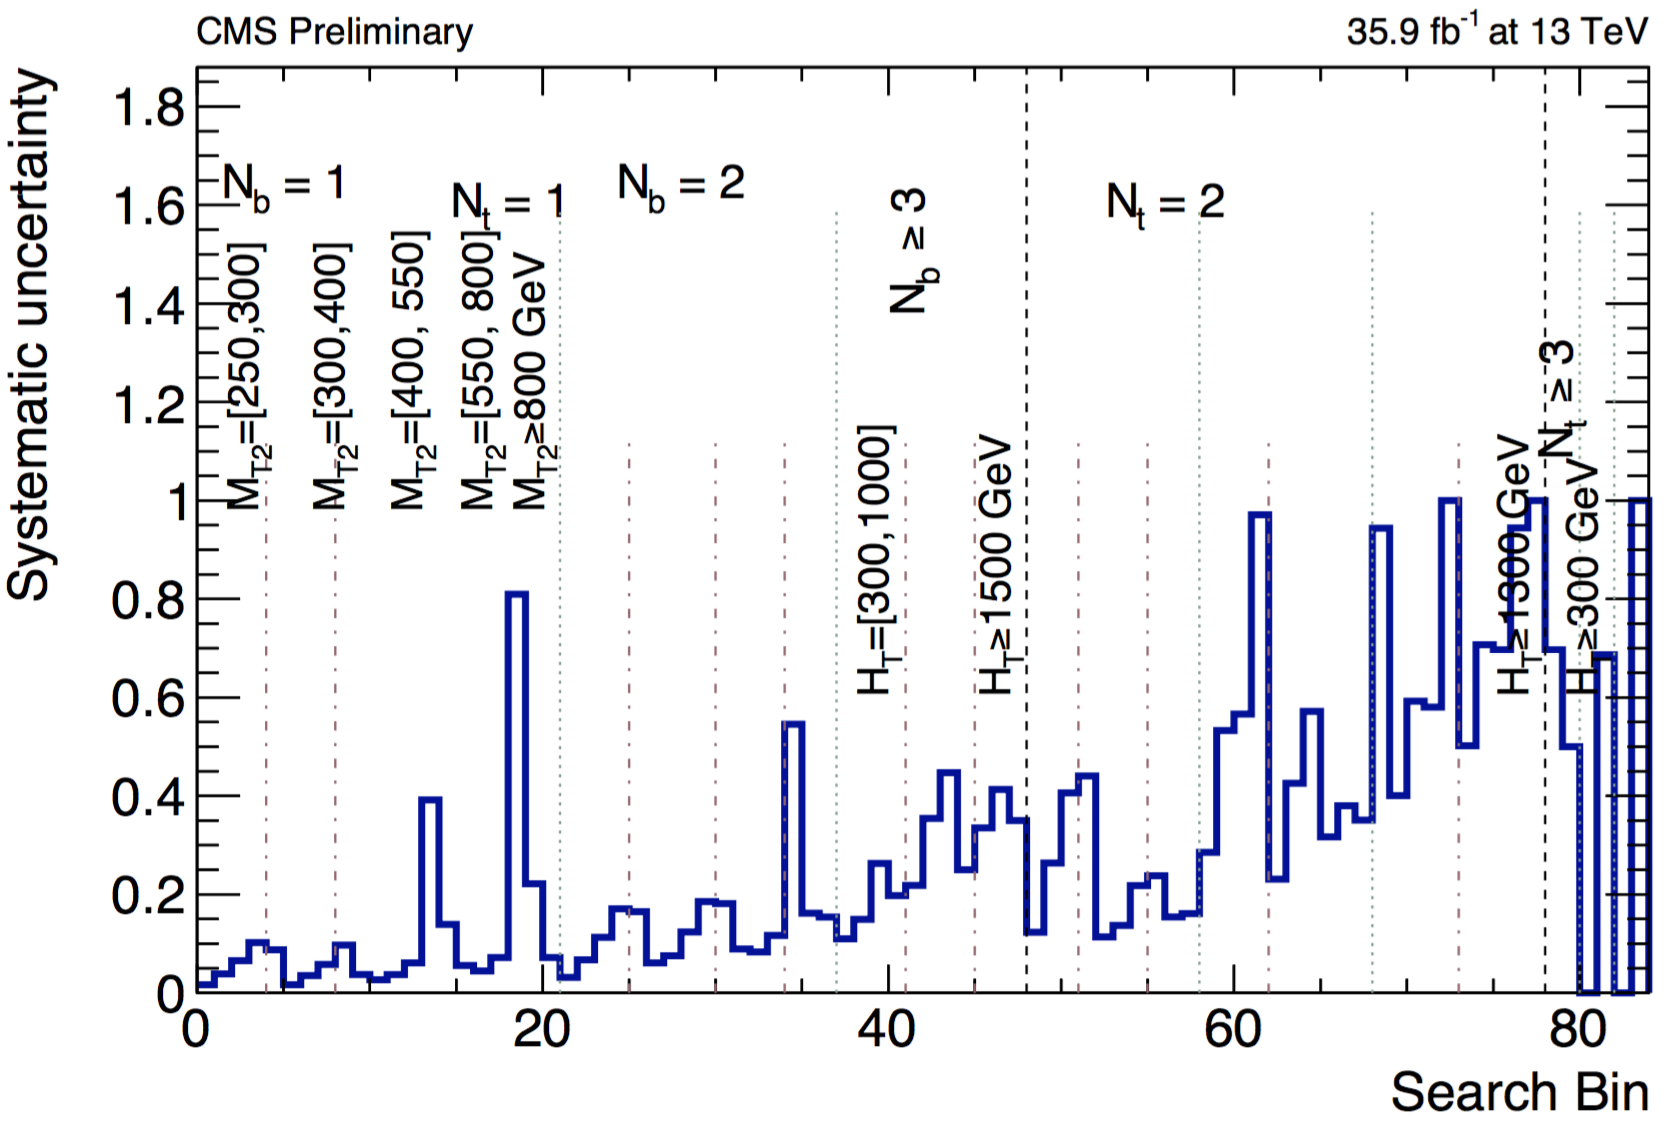
\includegraphics[width=0.8\textwidth]{UncZnunu}
\end{center}
\vspace{-1em}
\caption{Systematic uncertainty in the final prediction, as a function of the search bin, associated to the MC statistics.}
\label{UncZnunu}
\end{figure}

The statistical uncertainty associated with each bin in the MC is propagated as a systematic uncertainty. The relative uncertainty per bin can be see in \autoref{UncZnunu}. It shows that the uncertainties for the MC vary from as low as 1\% up to 81\% and even 100\% in some regions. Since the final estimation is scaled using the global normalization factor from the tight $\mu\mu$ control region ($R_{norm}$), the total uncertainty, due to limited amounts of events in data, is propagated in the final prediction. This is also true for the $S_\gamma$($N_j$) scale factor, in which the residual differences in search variables other than $N_j$ are evaluated in the loose photon control region. Both the uncertainty arising from the $N_j$ re-weighting as well as the residual differences are evaluated together. The uncertainty from $R_{norm}$ is propagated as a flat value of 7.9\% uncertainty per each search bin.

\subsection{Z$\rightarrow\nu\bar{\nu}$ Estimation for the Search Bins}

The final estimation for the Z$\rightarrow\nu\bar{\nu}$ background calculated for all 84 search bins is shown in \autoref{results}. The statistical uncertainty in bins that have zero events is treated as the average weight (the sum of the weights squared over the weight) times the poisson error on 0 which is 1.8. This average weight is calculated on the basis of a relaxed cut in which $N_b \geq 2$ is required. For comparison, a cut in which $N_t > 2$ where two tops are fake for the Z$\rightarrow\nu\bar{\nu}$ is used.

\begin{figure}[H]
\begin{center}
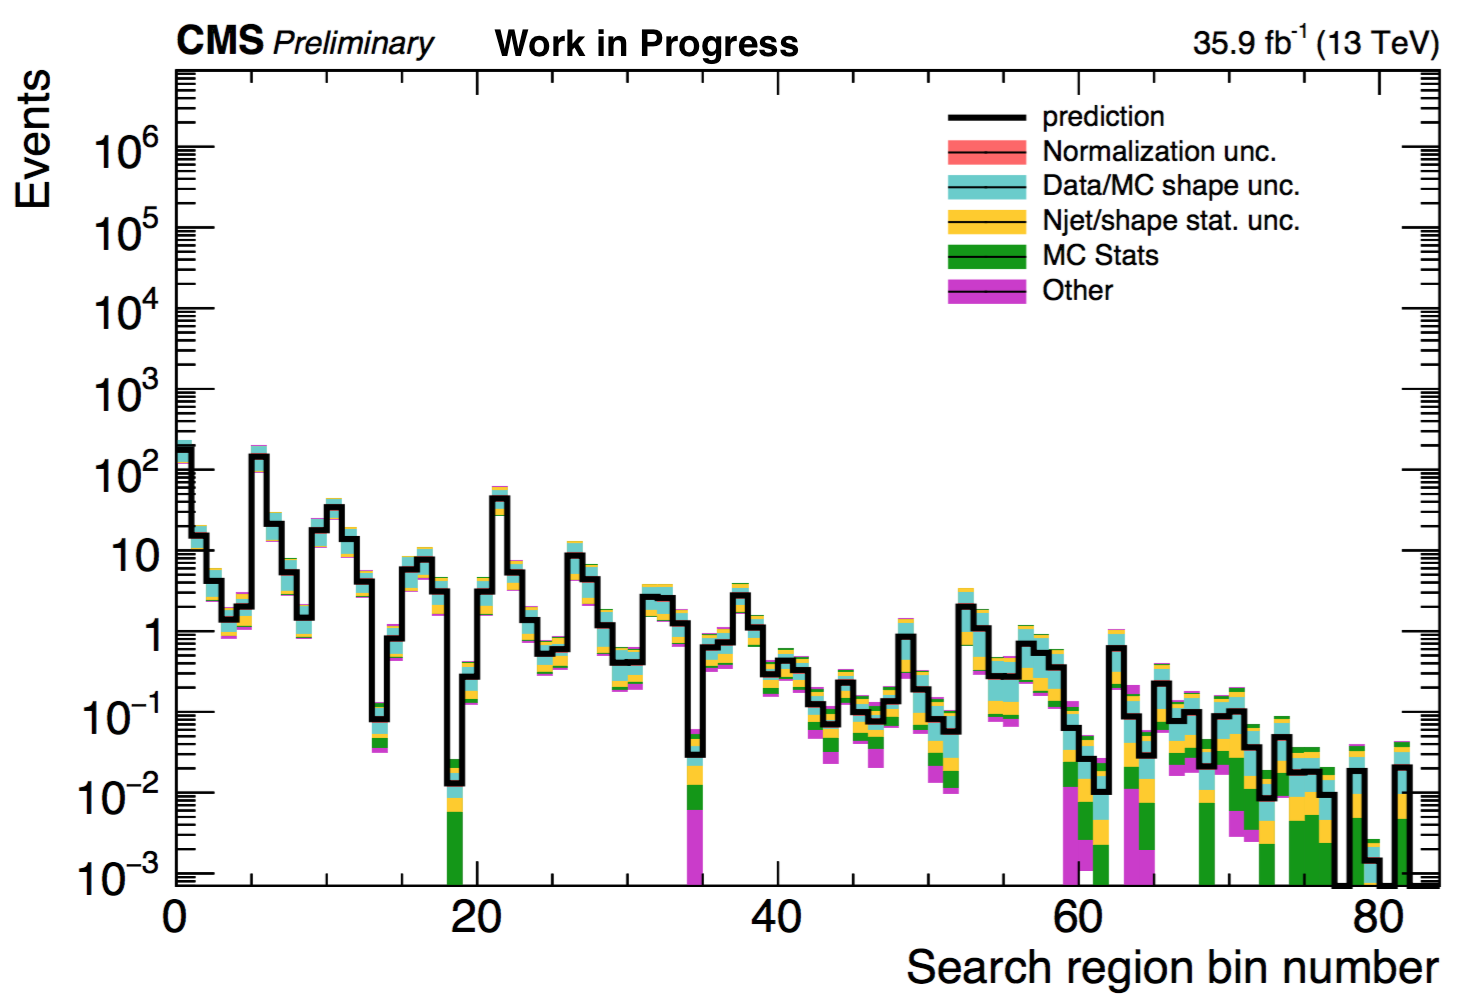
\includegraphics[width=0.8\textwidth]{Results.png}
\end{center}
\vspace{-1em}
\caption{Z$\rightarrow\nu\bar{\nu}$ background prediction for all search bins, including the breakdown of the various uncertainties.}
\label{results}
\end{figure}

